\section{Evaluation Design}
\label{sec:eval-design}

\subsection{Research questions}

\begin{description}[leftmargin=2.6em,style=nextline]
\item[\rqref{1} Identifiability in practice.] Does the anchored cell model recover interpreter accuracy and the defect form of each cell under realistic noise, and in which regimes does it beat simpler aggregators?
\item[\rqref{2} Effectiveness on seeded defects.] How accurately does \specdx detect, type and localise seeded defects, compared with seven published baselines?
\item[\rqref{3} Real defects.] Does \specdx rediscover the defects recorded in the subject's history?
\item[\rqref{4} Cost-effectiveness.] How does effectiveness grow with the number of runs, and how does \specdx compare with the baselines at equal cost?
\item[\rqref{5} Ablation.] What does each component contribute?
\end{description}

\rqref{1} is answered by simulation, which needs no GPU and has a known ground truth. \rqref{2}--\rqref{5} are answered on the subject specification.

\subsection{Subject}
\label{sec:eval-subject}

\Cref{tab:subject} summarises the subject, the procure-to-pay specification of TonomyX CASE-0031 (\cref{sec:motivating}). We vendored TonomyX byte for byte at a fixed commit and never edit it. \specdx has its own PostgreSQL instance. The subject is demanding for three reasons:
\begin{itemize}[leftmargin=*]
\item $\Tell$ is long, written in Vietnamese and spread over several documents;
\item $\Chk$ mixes declarative invariants, procedural SQL and a golden state;
\item the process involves human approval gates. At each gate, the scenario fixes the decision, and a persona interpreter records it and carries out its consequences.
\end{itemize}

\begin{table}[t]
\caption{The subject specification.}
\label{tab:subject}
\small
\begin{tabular}{@{}lp{10.6cm}@{}}
\toprule
Part & Content \\
\midrule
$\Tell$ & Business-analysis document (97 pp.), demo description (46 pp.), software architecture document (18 pp.), three knowledge-base articles, business principles, tool catalogue, schema, scope table and tool refusal messages; served through a BM25 retrieval tool \\
$\Chk$ & 42 invariants, scenario expectations, golden end state over 26 tables, guardrail triggers and SQL policy functions, blank-column list, event vocabulary, scope table; executed on PostgreSQL 16 through nine gated tools \\
$\Scen$ & Ordered quantity, received quantity, requested discount, receipts per order; three reference scenarios (\textit{happy}, \textit{discount8}, \textit{grn12}); T-boundary and synthesised scenarios \\
Process & Interpreter steps by digital employees and human-gate personas, from sales order to payment \\
\bottomrule
\end{tabular}
\end{table}

A second subject, the airline and retail domains of $\tau^2$-bench~\cite{barres2026bench} with the repairs of its verified release as real defects, is designed but not yet built. We return to it in \cref{sec:discussion}.

\subsection{Interpreter population}

The population is chosen by an automatic, outcome-free capability screen. Each candidate model runs the base specification on the \textit{happy} scenario under three Tell variants and three seeds. The screen measures two things:
\begin{itemize}[leftmargin=*]
\item the \emph{act rate}, the fraction of interpreter steps with $a_{bs}=1$;
\item the \emph{valid-call rate}, the fraction of tool calls that validate against the tool's schema.
\end{itemize}
The screen never compares a run with $\Chk$, because doing so would be circular when $\Chk$ is the object under diagnosis. A model is admitted when its act rate is at least $0.3$ and its valid-call rate is at least $0.8$. The ranking keeps at most two models per family and four in total, from at least two families. If fewer than four models are admitted, the study stops.

\Cref{tab:population} lists the admitted population. All models run locally through Ollama 0.30.4 with pinned weight digests.

\begin{table}[t]
\caption{Interpreter population chosen by the capability screen. Screen statistics are filled in from the frozen screen results.}
\label{tab:population}
\small
\begin{tabular}{@{}llrrr@{}}
\toprule
Family & Model & Parameters & Act rate & Valid-call rate \\
\midrule
Qwen & \texttt{qwen3:30b-a3b} & 30B (3.3B active) & \tbd & \tbd \\
Qwen & \texttt{qwen2.5:14b} & 14B & \tbd & \tbd \\
OpenAI (open weights) & \texttt{gpt-oss:20b} & 21B (3.6B active) & \tbd & \tbd \\
Mistral & \texttt{mistral-small3.2:24b} & 24B & \tbd & \tbd \\
\bottomrule
\end{tabular}
\end{table}

\subsection{Seeded defects}
\label{sec:eval-mutants}

We seed defects with nine specification mutation operators, listed in \cref{tab:operators}. In the spirit of specification mutation~\cite{black2000mutation,jia2011analysis}, every operator edits only artefacts that the running system reads, so every mutant takes effect. Every state-level operator also emits a \emph{kill witness}: a state that proves the defect is real and can be activated. This removes the equivalent-mutant problem~\cite{schuler2011assessing}.

Each operator declares the rows, fields or steps its truth needs to be observed (\textit{observed at}). This is benchmark metadata and is never an input to any method.

\begin{table}[t]
\caption{Specification mutation operators, application sites and the development/test split (five development mutants per type, stratified, fixed seed).}
\label{tab:operators}
\small
\begin{tabular}{@{}llp{7.4cm}rr@{}}
\toprule
Type & Op. & Edit & Sites & Truth location \\
\midrule
\multirow{2}{*}{\Dcon} & C1 & Add an invariant that conflicts with an existing row-level equality invariant (same row and column, different value) & 6 & clause pair \\
 & C2 & Add a guardrail trigger that forbids a status the golden state requires & 3 & clause set \\
\multirow{2}{*}{\Dhid} & H1 & Change a locked value in the golden state, with no support in $\Tell$ & 5 & golden clause \\
 & H2 & Add an invariant demanding an event that $\Tell$ never motivates & 2 & clause \\
\multirow{3}{*}{\Damb} & A1 & Delete a disambiguating sentence of $\Tell$ & 3 & chunk \\
 & A2 & Replace a precise value in a sentence of $\Tell$ by a vague phrase & 3 & sentence \\
 & A3 & Add a knowledge-base article with an overlapping validity period and a different cap & 1 & sentences \\
\multirow{2}{*}{\Dweak} & W1 & Remove a column from the blank list and delete the invariant that guards it & 7 & field \\
 & W2 & Delete a golden event that the interpreter is told to log & 6 & event \\
\midrule
\multicolumn{3}{@{}l}{Total: 36 mutants; development split 20 (5 per type); test split 16 (4\,/\,2\,/\,2\,/\,8)} & 36 & \\
\bottomrule
\end{tabular}
\end{table}

\paragraph{Scorability.} A mutant can be detected by \emph{any} behaviour-based method only if the population reaches the place it changes (\cref{prop:noaction}). A mutant is therefore \emph{scorable} when, in the base specification's runs, at least $k=3$ acted behaviours touch its \textit{observed-at} targets. The scorable set is computed once from base runs, before any mutant runs, and it is the same for every method. The primary tables score scorable mutants. Secondary tables score all mutants and report how many were excluded per type.

\subsection{Real defects}

\Cref{tab:real} lists the real defects. R-SO and R-12 were described in \cref{sec:motivating}.
\begin{itemize}[leftmargin=*]
\item \textbf{R-DE.} The list of digital employees declares 15 of them, while the scope table grants capabilities to only nine. The mismatch is a hidden requirement wherever $\Tell$ assigns work to an employee without scope.
\item \textbf{R-DOC.} A documentation-only inconsistency that no behaviour can expose. It is used only for a qualitative check of the static reviewer.
\end{itemize}

\begin{table}[t]
\caption{Real defects from the subject's history.}
\label{tab:real}
\small
\begin{tabular}{@{}lp{6.6cm}p{3.4cm}l@{}}
\toprule
Id & Defect & Expected type & Scored \\
\midrule
R-SO & \texttt{SO-0031} stays \emph{\vi{Chờ duyệt}} after \texttt{APR-0102} is approved, while \texttt{PO-0015} moves to \emph{\vi{Đã duyệt}} & \Dhid (mis-key) & yes \\
R-12 & The schema allows several receipts per order; \texttt{fn\_reconcile} raises a cardinality error on that input & \Dcon & yes \\
R-DE & 15 digital employees declared; 9 granted scope & \Dhid where $\Tell$ assigns such work & yes \\
R-DOC & README states 33 invariants, the invariant file has 42; load orders differ & documentation only & no \\
\bottomrule
\end{tabular}
\end{table}

\subsection{Baselines}
\label{sec:eval-baselines}

We compare \specdx with the closest published method for each defect type, or for each component of \specdx. \Cref{tab:baselines} lists them. Three candidates were excluded because their code carries no licence: ClarifyGPT~\cite{mu2024clarifygpt}, SpecFix~\cite{jia2025automated} and AgentSuite/COBA~\cite{suh2026agentsuite}. We discuss them in \cref{sec:related}.

\begin{table}[t]
\caption{Baselines. ``Runs'' means the baseline consumes exactly \specdx's cached runs of the same specification, including synthesised scenarios; any bias this introduces favours the baseline.}
\label{tab:baselines}
\small
\begin{tabular}{@{}lp{4.1cm}p{4.6cm}l@{}}
\toprule
Id & Method & Input and adaptation & Types \\
\midrule
B1 & BenchGuard~\cite{tu2026who} & Definition audit of instruction, tests and solution, packaged per specification; original package; open models & all four \\
B2 & Who\&When~\cite{zhang2025which} & Failing runs as multi-agent logs; three original strategies plus a ``specification defect'' verdict; open models & \Dhid \\
B3 & IRT audit, forced ceiling~\cite{land2026auditing} & Models $\times$ cells/clauses from runs; likelihood-ratio indicator & \Dhid \\
B4 & Semantic entropy~\cite{farquhar2024detecting,kuhn2023semantic} & Discrete entropy of cell readings (pooled and per family); same ddmin localiser as \specdx & \Damb \\
B5 & MUS on $\Chk$ alone~\cite{ignatiev2018pysat,liffiton2008algorithms} & Symbolic repair from the golden state, no interpreters; minimal hitting sets & \Dcon \\
TI & GLAD~\cite{whitehill2009whose}, Dawid--Skene~\cite{dawid1979maximum} & Task $=$ cell, worker $=$ model; flag when the aggregate $\neq d_c$ & \Dhid \\
JEST & $N{+}1$-version rule~\cite{park2021jest} & Flag a cell/clause when the share of deviating models $\ge\tau$ & \Dhid \\
\midrule
B2-naive & Best single interpreter & Every violated clause flagged (secondary arm) & \Dhid \\
B3-2PL & 2PL IRT~\cite{rodriguez2021evaluation} & Negative discrimination flagged (secondary arm) & \Dhid \\
\bottomrule
\end{tabular}
\end{table}

\subsection{Metrics}

\paragraph{Matching.} A typed detection requires both a type match and a location match:
\begin{itemize}[leftmargin=*]
\item \textbf{Hidden requirement:} the reported clause equals the true clause.
\item \textbf{Contradiction:} the Jaccard index between the reported clause set and the true conflict set is at least $0.5$.
\item \textbf{Ambiguity:} the reported sentence set intersects the mutated sentences. For a deletion, any reported sentence in the chunk that held the deleted sentence matches.
\item \textbf{Weak check:} the reported fields include the field whose guard was removed.
\end{itemize}
Untyped matching drops the type requirement. Findings that are also present in the base specification's report are removed before matching (the differential).

\paragraph{Measures.} For each type, we report typed precision, recall and $F_1=2\,\textit{tp}/(2\,\textit{tp}+\textit{fp}+\textit{fn})$, computed in exact arithmetic so that ties are exact. We also report two threshold-free measures: average precision (AP) and Detection@$k$ for $k\in\{1,3,5\}$. Cost is counted in model requests, the one unit common to every method. Tokens and GPU time are added where they were recorded. Runs cached before the request counter existed are charged an upper bound, which overstates \specdx's cost.

\subsection{Fairness protocol}
\label{sec:eval-fairness}

\begin{itemize}[leftmargin=*]
\item \textbf{Same inputs.} Every method runs on the same base specification and mutants, and the run-consuming baselines read exactly \specdx's runs.
\item \textbf{Same models.} B1 and B2 run on each of the four population models with their original generation settings, and every call goes through one cached gateway.
\item \textbf{Selection on development data only.} For each baseline, the model, the strategy and the reporting threshold are chosen on the base and the 20 development mutants. The rule maximises mean typed $F_1$ over the types the baseline reports, with ties going to the smaller model and then the higher threshold. The choices are then frozen and committed.
\item \textbf{Conservative asymmetry.} \specdx's own thresholds come from simulation only (\cref{sec:eval-sim}), while the baselines are tuned on real development data.
\item \textbf{Two cost views.} Table A compares every method at its native protocol. Table B compares each LLM-based baseline with \specdx at the anytime checkpoint (25, 50, 100, 150 or 200 population runs) whose cost is closest to, and not above, the baseline's. Recording checkpoints never changes the final report, and a test verifies byte-identity.
\item \textbf{One-shot test split.} The test split is run once, only after the development gate is passed and the baseline pre-registration is committed with a clean working tree. The pre-registration records the hash of the gate configuration and its result, and the study refuses to run on a mismatch.
\end{itemize}

\subsection{Pre-registered protocol}
\label{sec:eval-sim}

The study proceeds through four go/no-go steps. Each step's pass criterion was written down before the step ran. \Cref{fig:protocol} shows the order of the steps and the comparison study that follows them.

\begin{figure}[t]
\centering
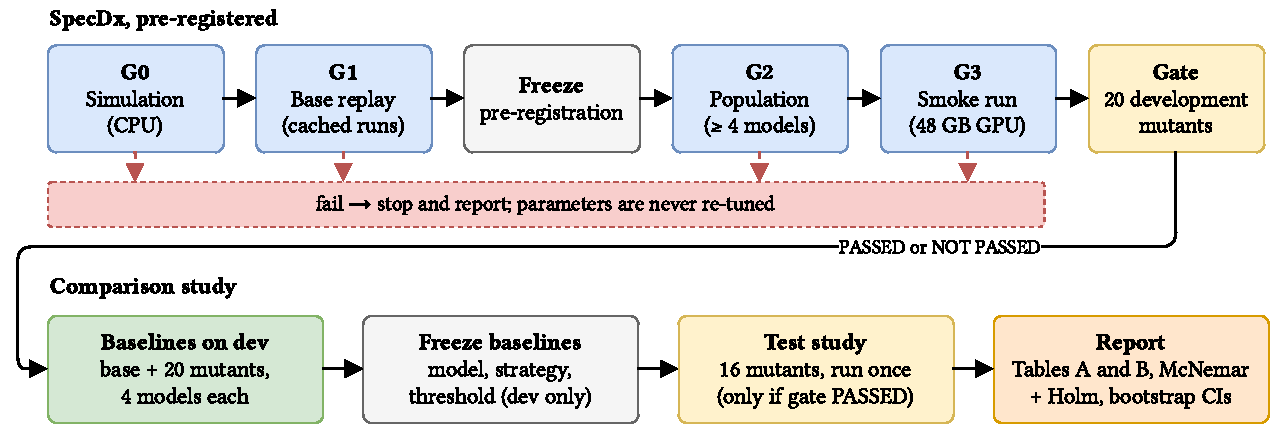
\includegraphics[width=\textwidth]{figures/drawio/protocol.pdf}
\caption{Evaluation protocol. Every go/no-go step has a pass criterion fixed in advance; a failure stops the study without re-tuning. The baselines are tuned on the development split whatever the gate's verdict, but the test split is run once, and only after the gate has passed and the baseline choices are frozen.}
\label{fig:protocol}
\end{figure}

\paragraph{G0: simulation.} We generate synthetic specifications with the following ingredients:
\begin{itemize}[leftmargin=*]
\item value and constraint cells, anchored and unanchored;
\item $M\in\{2,3,4\}$ models;
\item grouped difficulties, with an arm that spreads difficulty within groups;
\item Dirichlet errors, including concentrated ones;
\item planted defects of every form;
\item readings from three variants and three seeds, pooled over scenarios, with per-model act rates.
\end{itemize}
The generator is calibrated to summary statistics of base runs only, never to a mutant. The calibrated statistics are per-cell accuracy, dispersion, error concentration, act rates and readings per cell. Two \emph{misspecification arms} violate (A3), with model-specific errors, and (A5), with model-dependent silence.

The free parameters are chosen by a fixed rule: maximise mean simulated typed $F_1$ over hidden requirements, ambiguities and weak checks, at the calibrated point and the two arms with equal weight. Ties go to the more conservative setting.

G0 passes when all three criteria hold:
\begin{enumerate}[leftmargin=*,label=(\roman*)]
\item the mean $|\hat\theta_m-\theta_m|\le0.05$;
\item simulated typed $F_1\ge0.6$ for hidden requirements and $\ge0.4$ for ambiguity;
\item \specdx is never more than $0.05$ below the best simple baseline on any type, at the calibrated point, under either arm, and at the population's own size and accuracy gap; and it beats that baseline on ambiguity by more than $0.05$ at the calibrated point.
\end{enumerate}
The simple baselines are majority vote over models, ``deviates from the anchor'', and our earlier joint-class latent model. The regime map crosses mean cell accuracy $\{0.6,0.7,0.8,0.9,0.95\}$ with accuracy gap $\{0,0.1,0.2\}$ and $M\in\{2,4\}$, with at least five replicates per point and ten at the calibrated point.

\paragraph{G1: base replay.} The frozen model is fitted on cached base runs. It must not collapse: $\theta_m\ge0.5$ for the two strongest models. It must also report R-SO as a hidden requirement whenever the cell is observable.

\paragraph{G2: population.} The screen must admit at least four acting models from at least two families.

\paragraph{G3: smoke.} The base specification runs on the GPU host with a budget of 60, and every model must reach $\theta_m\ge0.5$.

\paragraph{Development gate.} On the 20 development mutants, \specdx wins a type under two rules:
\begin{itemize}[leftmargin=*]
\item \textbf{Contradiction and hidden requirement:} its typed $F_1$ exceeds the \emph{untyped} $F_1$ of both B2-naive and B3-2PL. These baselines cannot assign types, so a typed comparison would be trivially won.
\item \textbf{Ambiguity and weak check:} its typed $F_1$ is at least $0.4$. These baselines cannot locate truths in $\Tell$ or in fields at all.
\end{itemize}
A type with fewer than three scorable mutants counts as a loss, and the gate passes with at least three wins out of four. The test split stays locked until the gate passes.

\subsection{Statistics}

Comparisons are paired per mutant. We use the exact McNemar test on typed detection, comparing \specdx with each baseline, with Holm correction across baselines, and report paired risk differences as effect sizes. Confidence intervals are 95\% bootstrap intervals over mutants, with 10{,}000 resamples and a fixed seed. Because the test split is small, we emphasise effect sizes and intervals over $p$-values.

\subsection{Implementation and environment}

\specdx is implemented in Python 3.13. Inference uses NumPy. Hitting sets use PySAT~\cite{ignatiev2018pysat}, and the truth-inference baselines use crowd-kit~\cite{ustalov2024learning}. The implementation has an extensive unit and integration test suite. Every run is cached in an append-only log, keyed by the specification, the scenario, the interpreter and the model's weight digest, so that every table can be regenerated from raw logs.

Simulation, G0 and G1 run on a CPU. Interpreter runs use a single 48\,GB GPU with Ollama 0.30.4 and two parallel workers.
